\documentclass[usegeometry=true]{scrartcl}
\usepackage[ngerman]{babel}
\usepackage[T1]{fontenc}
\usepackage{lmodern}
\usepackage[utf8]{inputenc}
\usepackage{hyperref}
\usepackage{amssymb}
% Dimensionen bitte nicht ändern. 
\usepackage[left=2cm, right=2cm, top=2cm, bottom=2cm, bindingoffset=1cm, includeheadfoot]{geometry}
%Zeilenabstand bitte nicht ändern
\usepackage[onehalfspacing]{setspace}
%grafik einfügen
\usepackage{graphicx}
%einfügen von hyperref
\usepackage{hyperref}

\usepackage[backend=biber,style=numeric,]{biblatex}\addbibresource{literatur.bib}

\begin{document}
% ----------------------------------------------------------------------------
\subject{Projektbericht zum Modul Information Retrieval und Visualisierung Sommersemester 2022}
\title{Visualisierung des Datensatzes Student Behaviour}
%\subtitle{Untertitel}% optional
\author{Paul Tebbe, Matrikelnummer: 216237588}% obligatorisch
\date{21.12.2022}
\maketitle% verwendet die zuvor gemachte Angaben zur Gestaltung eines Titels
\pagebreak
% ----------------------------------------------------------------------------
% Inhaltsverzeichnis:
%\tableofcontents
% ----------------------------------------------------------------------------
% Gliederung und Text:

\section{Einleitung}
\label{Einleitung}
......
Viele verschiedene Faktoren haben einen Einfluss auf die Note der Studenten. Dies geht bereits damit los in welche Familie das Kind hineingeboren wird, welchen akademischen Standart die Eltern haben, welche finanziellen Mittel usw. Weiter spielt die Erziehung und der spätere soziale Umgang eine Rolle. \cite{Earthman}
Diese Einflüsse sind schwer zu messen, vor allem schwer genau zu messen. Diese Faktoren sind kaum von alleine beeinflussbar, es lässt sich nicht bestimmen, in welche Familie ich geboren werde und welche Voraussetzungen ich also für später mit auf den Weg gegeben bekomme. Doch auf welche Faktoren kann der Student selber später Einfluss nehmen. Die Zeit, die täglich in oder eben nicht in die schulische Weiterbildung investiert wird, sollte in der Theorie so einen selbst beeinflussbaren Faktor darstellen. 
In dieser Arbeit werden sich also folgende Fragen und folgende gestellt Zielstellungen gesetzt:

\begin{itemize}
\item Wie korrelieren Noten und Zeitgestaltung und lassen sich daraus Rückschlüsse ziehen, wenn ja welche? 
\item Wie stehen die Noten im Zusammenhang mit anderen Variablen?
\item Wie können die verschiedenen Daten übersichtlich veranschaulicht werden um dem Leser einen schnellen Überblick zu geben
\end{itemize}



Tipps zu Latex und Koma-Script für Hausarbeiten sind im \href{http://mirrors.ctan.org/info/latex-refsheet/LaTeX_RefSheet.pdf}{LaTeX Reference Sheet for a thesis with KOMA-Script} von Marion Lammarsch und Elke Schubert zusammengefasst. 
Der Bericht fällt in die Kategorie von InfoVis-Paper, die Tamara Munzner Design Study nennt \cite{Munzner2008}: In der Einleitung sollen sie zuerst das Zielproblem beschrieben. Daraus sollen sie Fragestellungen motivieren, die mittels Techniken der Informationsvisualisierung beantwortet werden können. In dem Abschnitt direkt unter der Überschrift Einleitung sollen Sie nach einer kurzen Einleitung Fragestellungen und das Zielproblem motivieren und beschreiben. ...

\subsection{Anwendungshintergrund}
Wer in der Schule und im College gute Noten hat und sich somit einen besseren Abschluss erarbeitet hat im späteren Leben deutlich bessere Chancen auf \glqq individuelle Lebenschancen, Selbstverwirklichung, beruflichen Erfolg sowie soziale, politische und kulturelle Teilhabe. \grqq
%\citep{Solga, Dombrowski 2008}





\subsection{Zielgruppen}
Die Zielgruppe für die Daten umfasst ein weites Spektrum an Personen. Die Visualisierung sind sowohl für Schüler und Studenten, als auch für Lehrer und Eltern interessant, also jegliche Personengruppe, die Berührungspunkte mit der Notengebung und deren Einflussfaktoren aufweist.
Die Informationen, die aus den Visualisierungen gewonnen werden können, können sehr gut dafür genutzt werden zu sehen, wie grade der Einflussfaktor Lernzeit und auch die vorangegangen Noten aus der Schulzeit einen Einfluss auf die Noten im College nehmen. Differenziert werden kann hierbei auch nochmal unter den Geschlechtern. 
Auch interessant könnte dieses Projekt aber auch für Forschende im Bereich soziale Ungleichheitne in der Bildung sein. Wenn keine eindeutigen Anzeichen zu sehen sind für eine Korrelation zwischen investierter Lernzeit und besseren Noten, so könnte dies ein Anzeichen dafür sein, dass doch andere Einflussgrößen mehr Auswirkung auf die Noten haben als der reine Fleiß. Dies wäre ein starker Indikator für soziale Ungleichheiten bei der Bildung, wie es bereits in der Einleitung angedeutet wurde. 



Beschreiben sie die Personengruppe oder Personengruppen, die das von ihnen benannte Anwendungsproblem lösen möchte. Auf welches Vorwissen können sie in dieser Gruppen von Anwenderinnen aufbauen? Welche Informations"-bedürf"-nisse werden durch die Visualisierungen adressiert?
\subsection{Überblick und Beiträge}
Der in dieser Arbeit verwendete Datensatz differenzieren die Studenten nach verschiedenen Merkmalen. Diese gehen von allgemeinen Unterscheidungen, wie Geschlecht, Alter und Gewicht, über die Aufteilung ihrer Freizeit und die aufgewendete Lernzeit bis hinzu dem körperlichen Wohlbefinden ausgedrückt mittels der Variable \glq stress level \grq .



\noindent Die für diese Visualisierung mit am interessantesten Daten sind die der verschiedenen Noten in der Schule und im college. Die Noten, gerade mit der von den Studenten angegebenen täglich Lernzeit sollte in einem positiven Zusammenhang stehen. Also steigt die Lernzeit am Tag, steigt auch die Note. Das gleiche sollte auch für die Beziehung der Noten untereinander gelten, also welcher Student schon in der 10.ten und 12.Klasse gute Noten hatte, sollte nun auch im College gut abschneiden. 
\noindent Die körperlichen Voraussetzungen sowie das Department sollten eigentlichen keine größeren Einflüssen auf die Noten haben.
\noindent Die Zeit verbracht auf sozialen Medien könnte eine negative Korrelation mit den Noten aufweisen, genauso wie der finanzielle Status und das Stress Level bei den Studenten.

In diesem Abschnitt geben sie einen kurzen Überblick über die Daten und verwendeten Visualisierungen. Dann benennen sie die Beiträge ihres Projekts. Diese Beiträge müssen sie in den hinteren Teilen des Berichts genauer ausführen und belegen.

\section{Daten}

Wie bereits in den Abschnitten vorher erwähnt, handelt es sich bei den vorliegenden Daten um den Datensatz \textit{Student Behaviour} von \textit{kaggle} . Die darin aufgeführten und gesammelten Daten geben nähere Auskunft über das Verhalten der Studenten und deren Noten. Die Verwendung des Datensatzes zu wissenschaftlichen Zwecken ist abzuraten, da der Verfasser angibt die Daten selber von Universitäten gesammelt zu haben und bis auf diesen Satz keine näheren Informationen zur Datenbeschaffung liefert. Seiner Meinung nach kann der Datensatz dazu genutzt werden das Verhalten der Studenten in Zukunft besser zu deuten.\\
Im Datensatz auf \textit{kaggle} sind ein paar Rechtschreibfehler bei der Variablenbenennung enthalten, wie z.B. \glqq social medai time\grqq , diese werden daher der Leserlichkeit halber im Folgenden grammatikalisch korrekt geschrieben)
\\
Er enthält Informationen von 235 Studenten in Form einer CSV-Datei. Diese CSV-Datei hat 19 Spalten mit den Informationen der Studenten über \textit{Certification} als Boolean, der ausgibt ob der Student einen certification Kurs besucht hat oder nicht, \textit{Gender} mit Boolean über das Geschlecht, \textit{Department}, welcher Student welchem Derpartment angehört, \textit{Height(CM)} und \textit{Weight(KG)} als Float, die Größe und Gewicht aufzeigen, \textit{10th Mark}, \textit{12th Mark} und \textit{College Mark}, die als Float die Note der Studenten zeigen, \textit{Hobbies}, sowie \textit{stress level} und \textit{financial status} als String, \textit{part-time job} und \textit{Do you like your degree} als Boolean, \textit{salary expectation} als integer (in Elm allerdings als Float deklariert und verwendet, damit es passend visualisiert und gemapt werden kann), \textit{willingness to pursue a career based on their degree } als String in Form einer Prozentangabe (möglich sind hier nur die Angaben: 0,25,50,75 und 100 Prozent) und \textit{travelling time}, \textit{social media time} und \textit{daily studying time} als String in Form einer Klassenangabe (also z.B. 30-60 Minuten ist eine Angabe).

Während sich grade die Noten, also 10th Mark, 12th Mark und College Mark sehr gut dazu eignen die Fragestellung zu beantworten und sich zusätzlich dazu noch gut visualisieren lassen, da sie als Float sich relativ einfach veranschaulichen lassen ist dies bei anderen Variablen weniger der Fall. Bei ein paar der Daten ist nichteinmal genau klar, was damit überhaupt ausgesagt werden soll, wie z.B. bei Certification Course. Was für ein Kurs ist das,  was zertifiziert man damit, bzw. welche Art von Zertifikation erwirbt man damit. Aufgrund des fehlenden Hintergrundwissen, welches leider im Datensatz nicht näher erläutet wird, kann bei diesen Visualisierungen nicht näher darauf eingegangen werden. Ähnlich verhält es sich bei Department. Auch hier fehlen die nötigen zusätzlichen Informationen, um diese Variable in geeigneter Weise einbauen zu können.
Auch die meisten Boolean (part-time job, Do you like your degree,  werden bei den Visualisierungen nicht berücksichtigt (bis auf gender), da es sich, bei den hier verwendeten Darstellungen nicht anbietet boolsche Werte zu integrieren. Diese bieten schlichtweg zu wenige Möglichkeiten.
Vielseitig genutzt wurde auch die daily studying time, die sich vor allem als \textit{drop-down} zur Sortierung der Noten eignete, sodass schnell ersichtlich wurde mit welcher Lernzeit welche Noten erreicht wurden. 
Hier wurde also eine der oben gestellten Zielstellungen sinnvoll und gut umgesetzt.

\subsection{Technische Bereitstellung der Daten}
\label{Bereitstellung}

Die Daten wurden als einzelne CSV-Datei in \textit{kaggle} bereitgestellt und auch also solche weiterverarbeitet. 
Zudem wurden sie im eigenen Github hochgeladen und dort im Ordner Daten gespeichert. Mithilfe dieser Datei wurden der Scatterplot und der Paralleplot erstellt. zur Visualisierung des Baumdiagramms wurde zusätzlich eine json-Datei erstellt \textit{"json.Name"} und auch im Ordner Daten hinterlegt. Zusätzlich dazu finden sich im Github-Repository auch noch Python-Code, mit dessen Hilfe die Daten aufbereitet werden sollen, genaueres in \ref{Datenvorverarbeitung}


\subsection{Datenvorverarbeitung}\label{Datenvorverarbeitung}
Im obigen Abschnitt wurde bereits kurz auf den Datensatz eingegangen und erklärt, dass es sich um eine einzelne CSV-Date handelte. Aufgrunddessen musste keinerlei größere Vorverabeitung an den Daten vorgenommen werden, zumindest für den Paralleplot und den Scatterplot. Für das Baumdiagramm wurde zuerst versucht mithilfe von Pyhtoncode die csv-Datei in eine json-Datei umzuwandeln. Leider gelang dies nicht, sodass die csv erst in eine Excel-Datei umgewandelt wurde. Anschließend wurde mithilfe der Excel-Datei manuell eine json-Datei erstellt um anhand dieser die Baumdarstellung zu visualisieren. In der json wurden dann nur die für das Baumdiagramm relevanten Daten übernommen. Aufgrund anfänglicher Überlegungen die verschieden klassierten \textit{Zeiten}, wie \textit{daily studying time}, \textit{social media time} und \textit{travelling time} in einzelne Klassen in Form von Integers festzuhalten, also \textit{daily studying time} von 0-30 Minuten wäre 1, 30-60 Minuten 2 usw. wurde die csv-Datei in R geladen um die Daten somit zu manipulieren. Aufgrund der späteren Nutzung der \textit{daily studying time} als Drop-down Tabelle wurde dieser Gedanke wieder verworfen.
%Zusätzlich Ausfilterung der Daten von SalaryExpectation aufgrund von Ausreißer
%Am Ende wurde dies aber dennoch erneut mit Pyhton gemacht allerdings mit den Daten \textit{social media time}, indem eine neue Spalte als daily studying class erstellt wurde und immer die Mitte der Zeit als Float erstellt wurde, sodass die Daten nun doch in den Parallelplot und den Scatterplot eingefügt wurden
\\

\section{Visualisierungen}
In den nachfolgenden Abschnitten wird näher auf die oben genannten Zielstellungen eingegangen.

\subsection{Analyse der Anwendungsaufgaben}
Wie bereits in \ref{Einleitung} erwähnt, sollen die folgenden Visualisierungen der Zielgruppe dabei helfen sich einen schnellen und übersichtlichen Eindruck über den Zusammenhang der unterschiedlichen Noten und anderen Variablen machen. Also welche Variablen nehmen möglicherweise Einflüsse auf die Note oder stehen in einem Zusammenhang mit diesen. 
Die Leser:innen  sollen sehen können, wie sich die Noten verändern wenn sich gewisse Variablen verändern, also wie ändert sich die Notenverteilung, wenn sich die Lernzeit erhöht oder verringert, welche Individuen der Ausgewählten sind Männer, welche Frauen. Auch auf einen möglichen Zusammenhang der sich im Laufe der Zeit verändernden Noten soll mithilfe der Visualisierungen eingegangen werden. Sind Studenten, die in der 10. Klasse gute Noten hatten auch in der 12. Klasse und im College noch so gut und umgekehrt genauso: War ein Student mit schlechten Noten schon in der 10. und der 12. Klasse schlecht und hängen diese Dinge möglicherweise mit dem Lernaufwand zusammen. All diese Fragen können in anschaulicher und so auch schneller Art und Weise von den Beobachtern auf den unterschiedlichen Visualisierungen überblickt werden, mit Unterstützung von verschiedenen Drop-Down-Möglichkeiten und der Hover-Funktion (hier werden den Lesern in den Plots immer die Auskunft über das Geschlecht und in manchen Fällen noch weitere allgemeine Informationen geliefert) über den Punkten oder den Parallellinien.
Das normale mentale Modell, dass bei einem Menschen entstehen sollte, wenn er sich diese Fragen und Anwendungsaufgaben stellt ist, dass es eine positive Korrelation zwischen guten Noten in der Schule und guten Noten im College, als auch zwischen Lernzeit und guten Noten existiert. In den Köpfen der Anwender entsteht also ein stetiger Anstieg der durschnittlichen Notenverteilung, je mehr Lernzeit dazukommt und dies sollte auch in den Abbildungen zu sehen sein. Die Mentalen Modelle sind für die Verständlichkeit der Visualisierungen für Leser allerdings  kaum notwendig, da sie relativ simpel gehalten sind und es auch eine der oben gestellten Anforderungen an das Projekt war, eine gewisse Komplexität nicht zu überschreiten. Die mentalen Modelle unterstützen also mehr die Visualisierungen, als dass sie vorausgesetzt werden um sie zu verstehen.
Allerdings ist, wie schon im oberen Bereich der Hausarbeit erwähnt die Gleichung, die Noten beeinflusst ein hochkomplexes Konstrukt, welche von reinen Zahlen kaum abgebildet werden kann, dies muss den Beobachtern bewusst bleiben und verzehrt so möglicherweise das eigene mentale Modell, gerade wenn bedacht wird, dass es sich bei \textit{Student Behaviour} um einen sehr kleinen Datensatz von 236 Studenten und um keine wissenschaftliche Studie, sondern eigens erhobene Daten handelt. Verwirrend wäre dies vor allem , wenn Studenten mit einer geringen Lernzeit sehr gute Noten haben und Studenten mit höher Lernzeit sehr schlechte, die könnte also durchaus dazu führen, dass der Leser mit einer Diskrepanz zwischen seinem mentalen Modell und der abgebildeten Visualisierung konfrontiert wird.



\subsection{Anforderungen an die Visualisierungen}
\label{Anforderungen}
\noindent Da die Leser einschätzen sollen können, ob und wenn ja inwieweit eine Korrelation zwischen den verschiedenen Parametern mit Noten und Zeitaufwand besteht, war es wichtig diese Daten aufeinander abgestimmt, in jeweils einer Visualisierung darstellen zu können.\\

\noindent Der Leser sollte bei allen Visualisierungen die Möglichkeit haben nach dem Parameter Zeit zu differenzieren und sich am Ende die Noten von den unterschiedlichen Studenten aus den unterschiedlichen Klassen/College ausgeben zu lassen. Es sollte also erst eine grobe Differenzierung getroffen werden können, um sich nach dieser ersten Einteilung genauer mit den verschiedenen Noten auseinandersetzen zu können.\\

\noindent Weiterhin war es wichtig die Visualisierungen recht einfach zu halten und schnell erkennbar werden zu lassen, ob die verschiedenen Parameter korrelieren oder nicht. 
\noindent Die einzelnen Visualisierungen wurden daher auf den ersten Blick relativ simple gehalten. Die Plots bieten die Möglichkeit des Drop-Downs und stellen am Anfang daher eine einfache Methode für den Betrachter dar, sich durch die verschiedenen Optionen zu klicken, ohne ihn direkt am Anfang mit Darstellungen und Informationen zu überhäufen. Durch die Anzahl von drei Drop-Downs ist es ihm aber wiederum möglich eine große Anzahl an Auswahlmöglichkeiten zu treffen und die Daten sich in vielen verschiedenen Kombinationen anzeigen zu lassen. Bei den Plots bietet sich die zusätzliche Optionen über die Punkte bzw. Linien zu hovern und so noch mehr Informationen über den jeweilig ausgewählten Studenten zu erlangen.\\

\noindent Die Visualisierung sollte in conclusio also anfägnlich einfach und übersichtlich gehalten sein und bei mehr Interesse auch weiter Möglichkeiten bieten.\\

\noindent Daher wurde sich für den Anfang für den Scatterplot entschieden, der eine Visualisierung darstellt,die die meisten Menschen kennen und der eine schnelle Übersicht über die Daten liefert, als zweites für einen Parallelplot, der die ersten Anfänge des Scatterplots erweitert, indem alle Noten auf einmal zu sehen sind. Als letztes das Baumdiagramm, dass alle im bisher im Fokus stehende Daten abbildet. 
\subsection{Präsentation der Visualisierungen}
Präsentieren sie die visuelle Abbildungen und Kodierungen der Daten und Interaktionsmöglichkeiten. 
Sie müssen  begründen, warum und wie gut ihre Designentscheidungen die erstellten Anforderungen erfüllen. 
Weiterhin müssen sie begründen, warum die gewählte visuelle Kodierung der Daten für das zulösenden Problem passend ist.
Typische Argumente würden hier auf Wahrnehmungsprinzipien und Theorie über Informationsvisualisierung verweisen. 
Die besten Begründungen diskutieren explizit die konkrete Auswahl der Visualisierungen im Kontext von mehreren verschiedenen Alternativen. 
Machen sie hier nicht den Fehler, einfach nur Visualisierung aus den vorgegebenen Bereichen zu diskutieren, weil das in der Regel nicht sinnvoll ist.
Wenn sie sich für einen Scatterplot entschieden haben, ist ein Zeitreihendiagramm in der Regel keine Alternative.
Diskutieren sie also nicht einfach Zeitreihendiagramme, weil sie in den Anforderungenen an das Projekt neben Scatterplots stehen, sondern suchen sie nach echten alternativen Visualisierungen, die zum Aufbau eines vergleichbaren mentalen Modells führen. 
Diskutieren sie die Expressivität und die Effektivität der einzelnen Visualisierungen. 

Die eben beschriebenen Präsentationen und Begründungen sollen für jede der drei folgenden Visualisierungen durchgeführt werden. 


\subsubsection{Visualisierung Eins}
Wie bereits in \ref{Anforderungen} erwähnt wurde sich als erste Visualisierung für den Scatterplot entschieden, abgebildet in Abbildung \ref{Scatter}.



\begin{figure}[h]
\begin{center}
	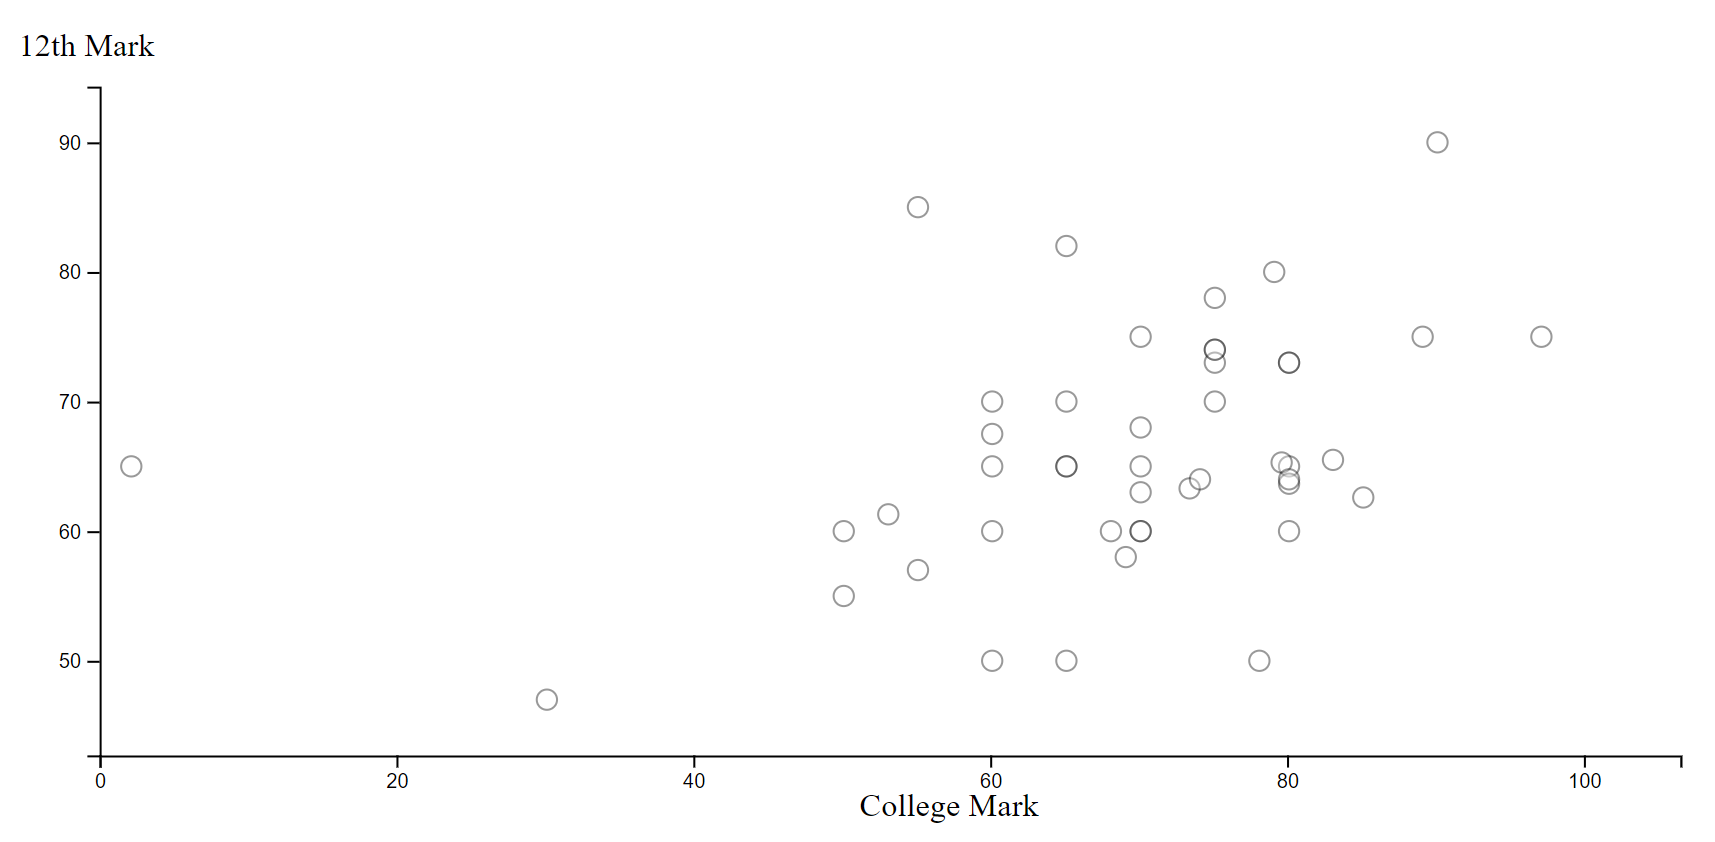
\includegraphics[scale=0.35]{Scatterplot.png}
	\caption{Scatterplot}
	\label{Scatter}
\end{center}
\end{figure}



Warum sich für den Scatterplot entschieden wurde, wurde bereits in \ref{Anforderungen} erläutert, zur genaueren Definition des Scatterplots und wie die \textit{Student Behaviour}-Daten darin dargestellt wurden wird in den folgenden Abschnitten näher darauf eingegangen.
\pagebreak
Der Scatterplot an sich besitzt zwei Achsen, die X-Achse und die Y-Achse. Deren Größe kann entweder manuell bestimmt werden oder hat vier weitere Möglichkeiten gleiche Daten verschieden darzustellen(\cite{Hinneburg2022})\\
\begin{itemize}
\item  X- und Y-Achse haben einen gleich großen Wertebereich
\item Nur die Y-Achse hat einen großen Wertebereich
\item Nur die X-Achse hat einen großen Wertebereich
\item Der Wertebereich in X und Y wird durch die Daten bestimmt
\end{itemize}

Die manuelle Einstellung der Achsen wäre sehr großer Aufwand und auch durchaus ungeeignet, weswegen sich hier für eine dynamische Option entschieden wurde.Die beiden Achsen wurden dem Wertebereich angepasst und können so auch flexibel mit den unterschiedlichen reingeparsten Daten interagieren und sich verändern. In Abbildung \ref{Scatter} enthält in diesem Beispiel die X-Achse als Werte die Daten von College Mark und die Y-Achse die Werte der Daten von 12th Mark.
Zusätzlich zu den dargestellten Achsen und deren Beschriftung enthält ein Scatterplot Punkte, die die verschiedenen zu untersuchenden Individuen und ihre Werte abbilden sollen (in diesem speziellen Fall die Studenten.\\
Aus dem Scatterplot kann also anhand der zwei beschrifteten Achsen und den Punkten auf einen Blick erkannt werden, wie die Notenverteilung bei den unterschiedlich ausgewählten Lernzeiten aussieht.\\

\noindent Wie bereits oben erwähnt können die X- und die Y-Achse dynamisch gewählt werden, genauso wie der \glqq Filter\grqq ,der die Lernzeit auswählt und unter dieser Prämisse die Daten der Noten auswählt

\begin{figure}[h]
\begin{center}
	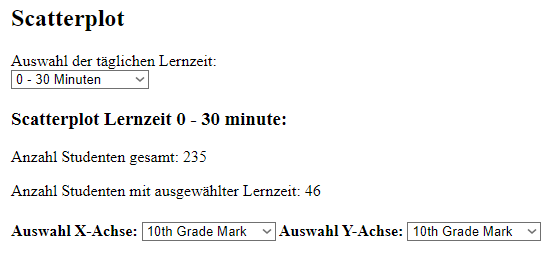
\includegraphics[scale=0.75]{ScatterDrop.png}
	\caption{Ausgewählte Drop-Down-Funktionen und Head}
	\label{ScatterDrop}
\end{center}
\end{figure}

Zu sehen in Abbildung \ref{ScatterDrop} ist, dass die Lernzeit 0-30 Minuten ausgewählt wurde und zusätzlich dazu die bereits erwähnten Achsen. So ist es dem LEser überlassen sich die verschiedenen WErte und differenten Korrelationen der Daten ausgeben zu lassen. Dies stellte eine der Anforderungen an die Visualisierung dar und wurde zusätzlich mit der einfachen Handhabung, gegeben durch die Drop-Downs in die Tat umgesetzt. Es lässt sich so sehr leicht auf einen Blick erkenne, in welchem Notenbereich sich Studenten bewegen, die 0-30 Minuten lernen. Zusätzlich dazu wird die Relation zwischen der Note im College und der Note aus der 12.Klasse abgebildet. \\
Dem Leser werden außerdem zwei zusätzliche Informationen geliefert, einmal wieviele Studenten es insgesamt gibt und außerdem wieviele Studenten von dieser Gesamtanzahl grade ausgewählt sind. Also wieviele Studenten von 235 0-30 Minuten lernen, in dem Fall 46. \\
So kann sich der Leser ein besseres Bild dazu machen, wie sich die Lernzeit grobt verteilt.\\
Außerdem wird dem Betrachter die Hover-Funktion bereitgestellt, dass bedeutet, dass wenn er über die einzelnen Punkte mit der Maus rüber fährt, leuchtet der Punkt grün auf und gibt ihm das Geschlecht mittig über dem Punkt aus.\\

\noindent Eine weiter ähnliche Visualisierungstechnik ist der QQ-Plot, dieser Teil die Datenwerte in verschiede Quantile ein. Hier werden die Verteilunen verglichen, Hinneburg beschreibt es als \glqq Verschiebungen zwischen zwei Verteilungen werden effizient durch Vergleich der Quantile gefunden\grqq \\
\cite{Hinneburg2022}. Da bei der zugrundeliegenden Arbeit allerdings nicht die Quantile veranschaulicht werden sollen, sondern vielmehr die einzelnen Noten der Studenten interessant sind, macht ein Scatterplot deutlich mehr Sinn.

\subsubsection{Visualisierung Zwei}
Die zweite Visualisierung wurde in Form eines Parallelplots dargestellt. Dieser hat, wie bereits in \ref{Anforderungen} gegenüber des Scatterplots den Vorteil, dass hier mehrere Daten auf einmal, sogenannte mehrdimensionale Daten dargestellt werden können.\\ Es können also von einem Studenten unter der Auswahl einer Lernzeitklasse alle Noten auf einmal darstellen. Hierzu werden die verschiedenen Attribute (Noten) vertikal nebeneinander aufgelistet und mithilfe einer Linie verbunden. Diese Linie übernimmt quasi die Aufgabe des Punkts aus dem Scatterplot und veranschaulicht so einzelne Studenten, siehe \ref{Parallel}. Hierbei wurde sich wieder für die Noten 10.Klasse, 12.Klasse \& College Mark zusätzlich zu \textit{Salary expectation} entschieden. So kann die mögliche Korrelation zwischen den einzelnen Noten und der Lernzeit und der Korrelation der einzelnen Noten untereinander gut veranschaulicht werden.\\



\begin{figure}[h]
\begin{center}
	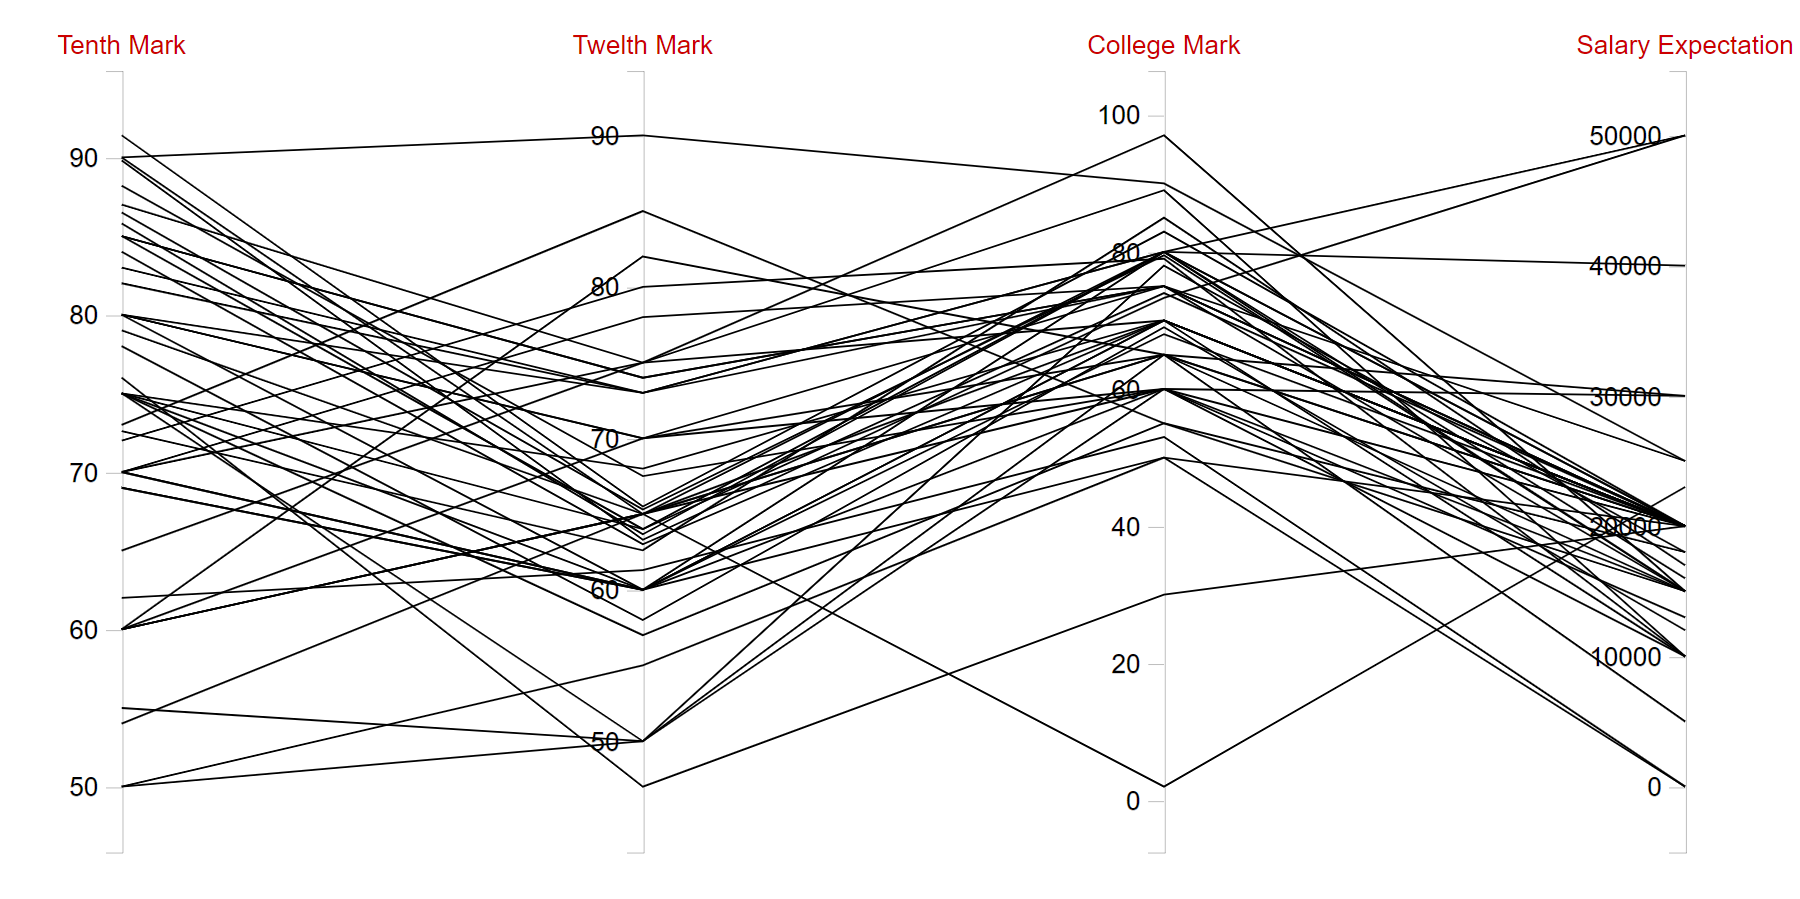
\includegraphics[scale=0.35]{ParallelPlot.png}
	\caption{Parallelplot}
	\label{Parallel}
\end{center}
\end{figure}

\noindent Der Leser erhält außerdem wieder als Kopf über der Visualisierung die Auswahl zwischen den einzelnen Lernzeiten per Drop-Down zu navigieren und erneut die Information, wie viele Studenten es insgesamt und wieviele Studenten es in der jeweils ausgewählten Zeitklasse gibt, siehe Abbildung \ref{ParallelDrop}. \pagebreak

%eventuell erwähnen, dass die Zeitangabe im Header auch dynamisch?

\begin{figure}[h]
\begin{center}
	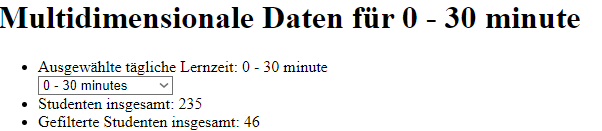
\includegraphics[scale=1]{ParallelDrop.png}
	\caption{Drop-Down Fenster und Head des Parallelplot}
	\label{ParallelDrop}
\end{center}
\end{figure}


\noindent Für den Leser ist so nun, wie in der Zielstellung in \ref{Einleitung} formulierten Anforderung auf einen Blick ersichtlich, wie sich die Verteilung der Noten gestaltet. Sollten sich sehr viele Linien im höheren Segment des Parallelplots ansiedeln, so ist klar, dass in der ausgewählten Lernklasse (in diesem Beispiel 0-30 Minuten)viele Studenten gute Noten in der Schule hatten und immer noch gute Noten im College haben, sowie eine hohe Erwartung an ihr späteres Gehalt haben. Genau das gleiche gilt selbstverständlich für den umgekehrten Fall.\\

Dem Vorteil der mehrdimensionalen Datendarstellung des Parallelplots steht allerdings die Ünubersichtlichkeit des Gleichnamigen gegenüber. Wenn auch alle Daten auf einmal abgebildet werden können, so leidet darunter die exakte Differenzierung der unterschiedlichen Individuen. Beim Parallelplot ist es also durchaus schwierig die einzelnen Studenten voneinander zu differenzieren, da die Linien sich an den unterschiedlich Abschnitten schneiden und so nicht genau erkennbar ist, wo welche Linie weiterführt. %daher einführung hover Funktion!

\noindent 





\subsubsection{Visualisierung Drei}



\subsection{Interaktion}
Die präsentierten Visualisierungstechniken müssen interaktiv zu einer Anwendung verknüpft werden.
Die Interaktion mit einer Visualisierung soll in den anderen Visualisierungen zu einer Änderung führen. 
Erklären sie die möglichen Interaktionen mit den einzelnen Visualisierungen und die möglichen Verknüpfungen zwischen ihnen. Begründen Sie warum die konkreten Interaktionen umgesetzt wurden und welche Zwecke für die Anwenderinnen mit ihnen unterstützt werden. Begründen sie ebenfalls warum sie andere Interaktionsmöglichkeiten nicht umgesetzt haben. Wenn sie keine der geforderten Interaktionen umsetzen, erhalten Sie im gesamten Projekt deutlichen Punktabzug. 

\section{Implementierung}
Beschreiben Sie die Implementierung ihrer Visualisierungsanwendung in Elm. Stellen die Gliederung ihres Quellcodes vor. Haben Sie verschiedene Elm-Module erstellt. Was war aufwändig umzusetzen, was ließ sich mit dem vorhanden Code aus den Übungen relativ einfach umsetzen? 

Wie sieht die Elm-Datenstruktur für das Model aus, in dem die verschiedenen Zustände der Interaktion gespeichert werden können.

\section{Anwendungsfälle}
Präsentieren sie für jede der drei Visualisierungen einen sinnvollen Anwendungsfall in dem ein bestimmter Fakt, ein Muster oder die Abwesenheit eines Musters visuell festgestellt wird. Begründen sie warum dieser Anwendungsfall wichtig für die Zielgruppe der Anwenderinnen ist. Diskutieren sie weiterhin, ob die oben beschriebene Information auch mit anderen Visualisierungstechniken hätte gefunden werden können. Falls dies möglich wäre, vergleichen sie die den Aufwand und die Schwierigkeiten ihres Ansatzes und der Alternativen. 
\subsection{Anwendung Visualisierung Eins}
\subsection{Anwendung Visualisierung Zwei}
\subsection{Anwendung Visualisierung Drei}

\section{Verwandte Arbeiten}
Führen sie eine kurze Literatursuche in der wissenschaftlichen Literatur zu Informationsvisualisierung und Visual Analytics nach ähnlichen Anwendungen durch. Diskutieren sie mindestens zwei Artikel. Stellen sie Gemeinsamkeiten und Unterschiede dar.

\section{Zusammenfassung und Ausblick}
Fassen sie die Beiträge ihre Visualisierungsanwendung zusammen. Wo bietet sie für die Personen der Zielgruppe einen echten Mehrwert.

Was wären mögliche sinnvolle Erweiterungen, entweder auf der Ebene der Visualisierungen und/oder auf der Datenebene?

\section*{Anhang: Git-Historie}

\printbibliography

\end{document}

